\chapter{A Brief Introduction to Stereoscopy}

The theoretical section serves to present a thorough literature review and build the 
theoretical framework for the entire study. Thorough concept definition is essential for 
the  reader  to  understand  what  the  author  intends.  It  is  important  that  the  theoretical 
section forms a coherent whole with the entire thesis. Secondary issues concerning the 
actual thesis are not presented in the theoretical section. The reader can be assumed to 
be  a  technology  professional  without  any  specialized  knowledge  of  the  topic  in 
question. Hence, it is not necessary to present basic issues in the Masters thesis. 
In  addition  to  the  theory,  the  background  information  in  many  cases  includes,  for 
instance, a company's old products, the system to be replaced, standards to be followed 
and a company's internal practices, and other parts of the project if the thesis is part of a 
larger  project.  These  are  presented  in  as  great  detail  as  is  necessary  to  expound  the 
solutions and provide a general view.  
More detailed outlining and headlining of the chapter (including the main heading) 
is  to  be  planned  and  written  according  to  the  requirements  set  by  the  thesis.  The 
Theoretical  background  or  Starting  points  chapter  can  also  be  divided  into  several 
sub chapters.   

\paragraph{}
We humans are gifted with a pair of eyes, which simultaneously captures rays of light and sends the 
information to our brain. The brain after some complex processing fuses them to create a three dimensional
(3D) map of the visible space. This 3D map is unique; it contains the approximate relative distance
of all the points in the scene with respect to the eye.

\paragraph{}
Thus, the photograph captured by a film or digital camera has one fundamental difference with the ones formed 
in the brain. The former is represented two dimensions (2D) i.e. height and width. It lacks the depth information, which in the field of computer vision (CV) is regarded as the third dimension.

\section{Depth cues}

\paragraph{}
Since, 3D viewing requires at least two light sensors, it is also regarded as stereoscopy. However, study
\cite{bib:stereo_cue} suggests, along with stereo vision the brain might use other cues to determine the relative distances and depth in a scene. These cues are gathered by only one eye and hence known as monocular (or extrastereoscopic) cues. 

\subsection{Monocular depth cue}
\paragraph{}
Monocular depth cues play a significant role in perception of depth. To an extent, the significance  depends on the distance between the observer and the scene. Some of the important ones are listed below.

\begin{itemize}
  \item \emph{Accommodation of the eye:} Human eye can change its optical power in order to focus on the object of interest. This is achieved by changing the form of the elastic lens. Even though this is mostly a reflex action but can be controlled to some extent manually.
  
  \item \emph{Relative size:} Objects which creates a bigger image on the retina is perceived to be closer.
  
  \item \emph{Relative height:} Objects placed higher in the scene generally tend to be perceived as further away.
  
	\item \emph{Overlapping of objects:} If one object is occluded by another, it is obvious that the occluding object is closer. This is also known as interposition.
		
	\item Linear perspective: The image of two parallel lines or edges, formed on the retina, seem to converge in such a way that they will eventually meet at infinity.
	
	\item \emph{Blur and desaturation:} When the eyes focus on an object it forms a sharp and a color rich image on the retina. The part of the scene that lies outside the focus plane appears to be blur. Desaturation i.e. converting to gray-scale, a part of a scene also gives the effect of out-of-focus region.
	
	\item \emph{Haze, De-saturation, and a shift to bluishness:} In the real world the light traveling from distant objects has to pass through dust or water vapor present in the air giving rise to such effects.
	
	\item \emph{Other cues:} Light, cast shadow and textured pattern are some of the cues commonly used to replicate 3D scene.
	
\end{itemize}

\subsection{Binocular depth cue}
\paragraph{}
The most important aspect here is that the eyes are separated from each other by a certain distance (about 64 mm in adults) called the inter-ocular distance. Thus we can observe two different perspective of the same scene. From this, the brain derives two important cues called convergence and retinal disparity shown in \textit{figure~\ref{fig:retinal_disparity}}.
 
\begin{figure}[ht]
\centerline{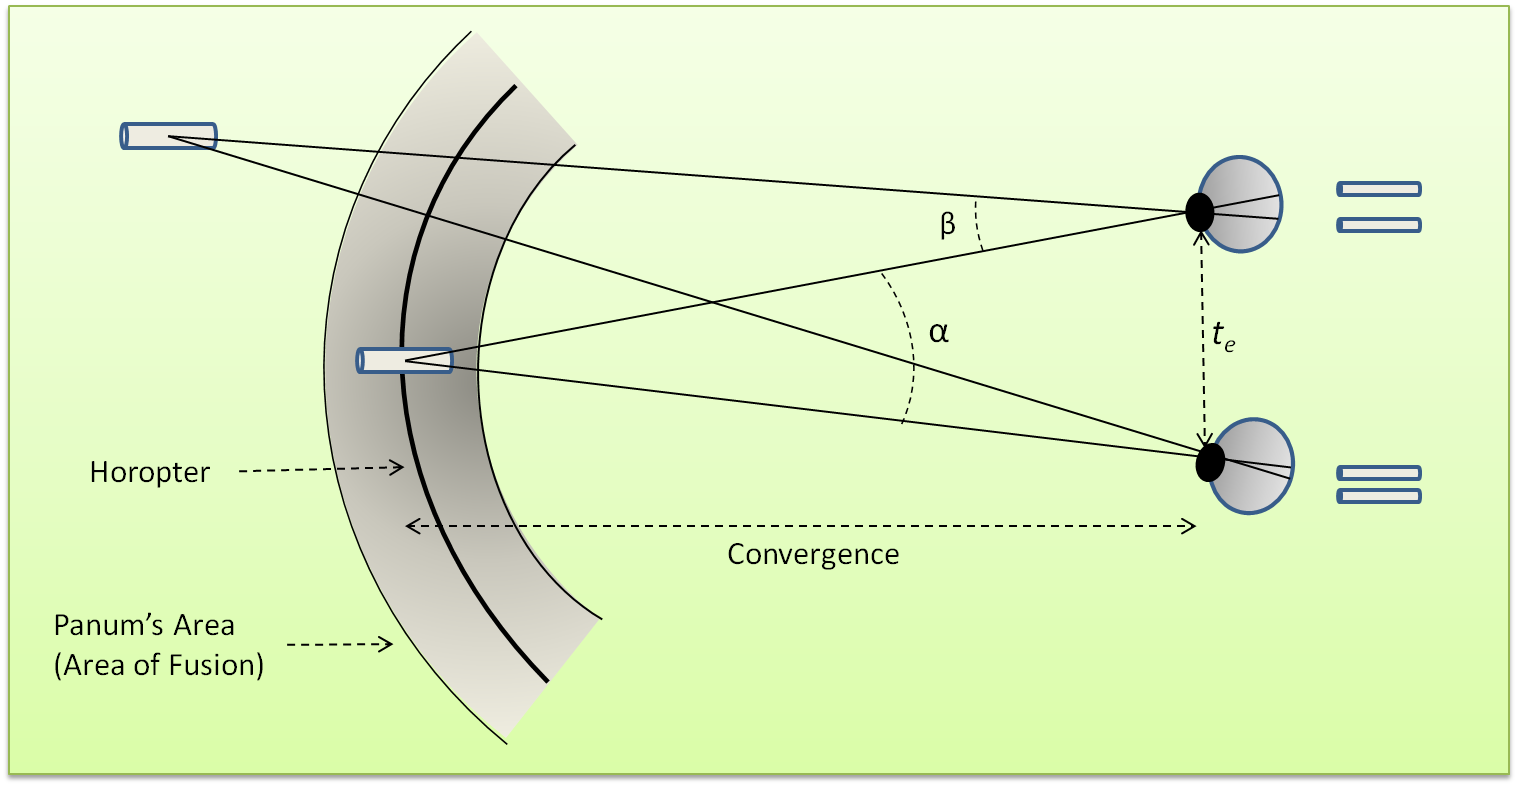
\includegraphics[width=1.0\textwidth]{retinal_disparity.png}}
\caption{\textit{Convergence and retinal disparity... \cite{bib:production_rules}} \label{fig:retinal_disparity}.}
\end{figure}

\paragraph{}
\emph{Vergence:} When the eyes tries to focus on an object it rotates the eye-ball such that the image is formed at the center of the retina. The angle of rotation is called the vergence angle $\beta$, as shown in the \textit{figure~\ref{fig:retinal_disparity}}. For near objects the eyes rotate towards each other and is known as convergence. The angle formed between the two optical axis is called convergence angle $\alpha$. They are related as $\beta = \alpha / 2$. Vergence assists the HVS to estimate the distance of the object to the eye.

\paragraph{}
\emph{Retinal disparity:} The object lying on the horopter forms an image on the center of the retina for both the eyes. However, the images formed for objects lying outside the horopter, has certain amount of disparity compared to each other (as shown in \textit{figure~\ref{fig:retinal_disparity}}). This is called retinal disparity or binocular parallax, and along with the angle of vergence, this gives an important cue for the brain to construct  3D image of the object and the environment surrounding it.

\subsection{Depth cues for 3D Displays}
\paragraph{}
Most commercially 3D displays available today are planostereoscopic devices. Such devices provides the viewer with a pair of images for left and right eye, on the same plane of the screen. These two images are exactly similar except that each point in one view has a corresponding point in the other view which is slightly displaced. This displacement or parallax provides enough cue for the brain to create an illusion of 3D. There are in fact three kinds of parallaxes (as shown in \textit{figure~\ref{fig:depth_parallax}}).

\paragraph{}
\emph{Positive parallax: }In this case the point in the the right-view lies on the right of it's corresponding point in the left-view (see \textit{figure~\ref{fig:depth_parallax}(a)}). Hence, the viewing rays seem to converge on the plane behind the screen. This gives an impression that the object lies in the screen space (for screen space see \textit{figure~\ref{fig:Stereoscopic_comfort_zone}}). To display an object located at infinity the displacement has to be equal to the inter-ocular distance; which means, it is the maximum possible disparity that can be produced on the screen.

\paragraph{}
\emph{Zero parallax: }In this case the left and right-view points is located at the same point. Thus the viewing rays seem to converge on the screen (see \textit{figure~\ref{fig:depth_parallax}(b)}).

\paragraph{}
\emph{Negative parallax: }Finally, for negative parallax, the point in the right-view lies on the left of it's corresponding point in the left-view (see \textit{figure~\ref{fig:depth_parallax}(c)}). Thus the viewing rays seem to converge at a point in front of the screen giving the impression that the object lies in the theater space (for theater space see \textit{figure~\ref{fig:Stereoscopic_comfort_zone}}).


\begin{figure}[ht]
\centerline{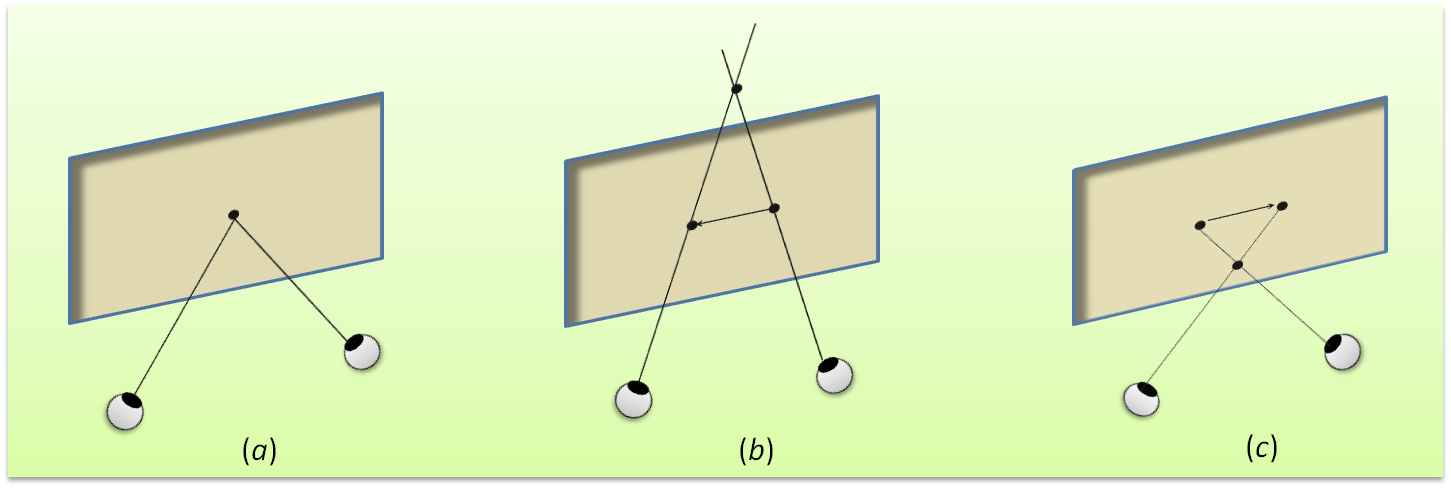
\includegraphics[width=1.0\textwidth]{depth_parallax.png}}
\caption{\textit{Disparity or Parallax for 3D viewing. (a) Positive parallax (b) Zero parallax (c) Negative parallax \cite{bib:production_rules}} \label{fig:depth_parallax}.}
\end{figure}


\section{Stereoscopic 3D}
\paragraph{}
In this thesis, we will deal with stereoscopic images. Such images are captured with two cameras which are synchronized and separated by a certain distance. Thus we obtain two images, left-view and right-view. 

\paragraph{}
A disparity map is computed from these two images. Each point may be considered as a two dimensional vector, which maps the corresponding points in the left and right view of a stereo pair. This is more commonly known as stereo matching or stereo correspondence and is discussed by D. Scharstein and R. Szeliski in \cite{bib:stereo_correspondence}.

\paragraph{}
Using the method of triangulation, a depth map is computed which indicates the relative distance of a point in the scene from the camera plane. Considering the disparity as $\emph{\textit{d}}$, base offset i.e. separation between the two cameras as $\emph{\textit{b}}$ and focal length to be $\emph{\textit{f}}$, the depth $\emph{D}$ can be calculated as

\begin{equation}
D = \frac{\textit{b} \cdot \textit{f}}{\textit{d}}
\end{equation}

\begin{figure}[ht]
\centerline{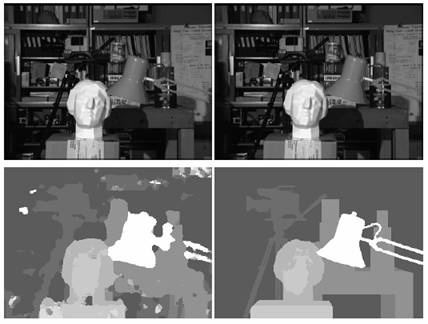
\includegraphics[width=0.8\textwidth]{stereo_disparity_depth.png}}
\caption{\textit{Top left and top right forms the two views of stereo pair. Lower left shows the unfiltered disparity-map and lower right shows the filtered disparity-map \cite{bib:img_stereo_disparity_depth}} \label{fig:depth_disparity}.}
\end{figure}


\paragraph{} 
However, given one view and an additional scene geometry like the depth map or disparity map, the other view can be reconstructed. The depth map is usually represented as a quantized 8 bit/sample (0 to 255) inverted range image i.e. 0 refers to the farthest point whereas 255 refers to the nearest. Since the range map is inverted the nearby objects have higher depth resolution.

\paragraph{}
The depth map is preferred, since unlike disparity, it is independent of the camera baseline i.e. the distance between the cameras, the camera sensors and image resolution.


\paragraph{}
Depth information can be obtained in different ways. High resolution depth information can be computed from a pair of intensity images using algorithms known as stereo correspondence or stereo matching. Another method is by using special sensors, like the time-of-flight cameras. However, he sensor based methods comes needs some post-processing owing to their low resolution, inaccurate estimation for larger distances and also due to the fact that the image sensor and the depth sensor are placed at slightly shifted location.  
	
\section{Depth-Image Based Rendering}
All work and no play makes Jack a dull boy,All work and no play makes Jack a dull boy,All work and no play makes Jack a dull boy,All work and no play makes Jack a dull boy,All work and no play makes Jack a dull boy...All work and no play makes Jack a dull boy, all work and no play makes Jack a dull boy, all work and no play makes Jack a dull boy.

\section{Encoding of depth map}
All work and no play makes Jack a dull boy,All work and no play makes Jack a dull boy,All work and no play makes Jack a dull boy,All work and no play makes Jack a dull boy,All work and no play makes Jack a dull boy...All work and no play makes Jack a dull boy, all work and no play makes Jack a dull boy, all work and no play makes Jack a dull boy.

\section{Issues related to Depth-maps}
All work and no play makes Jack a dull boy,All work and no play makes Jack a dull boy,All work and no play makes Jack a dull boy,All work and no play makes Jack a dull boy,All work and no play makes Jack a dull boy...All work and no play makes Jack a dull boy, all work and no play makes Jack a dull boy, all work and no play makes Jack a dull boy.

\begin{figure}[ht]
\centerline{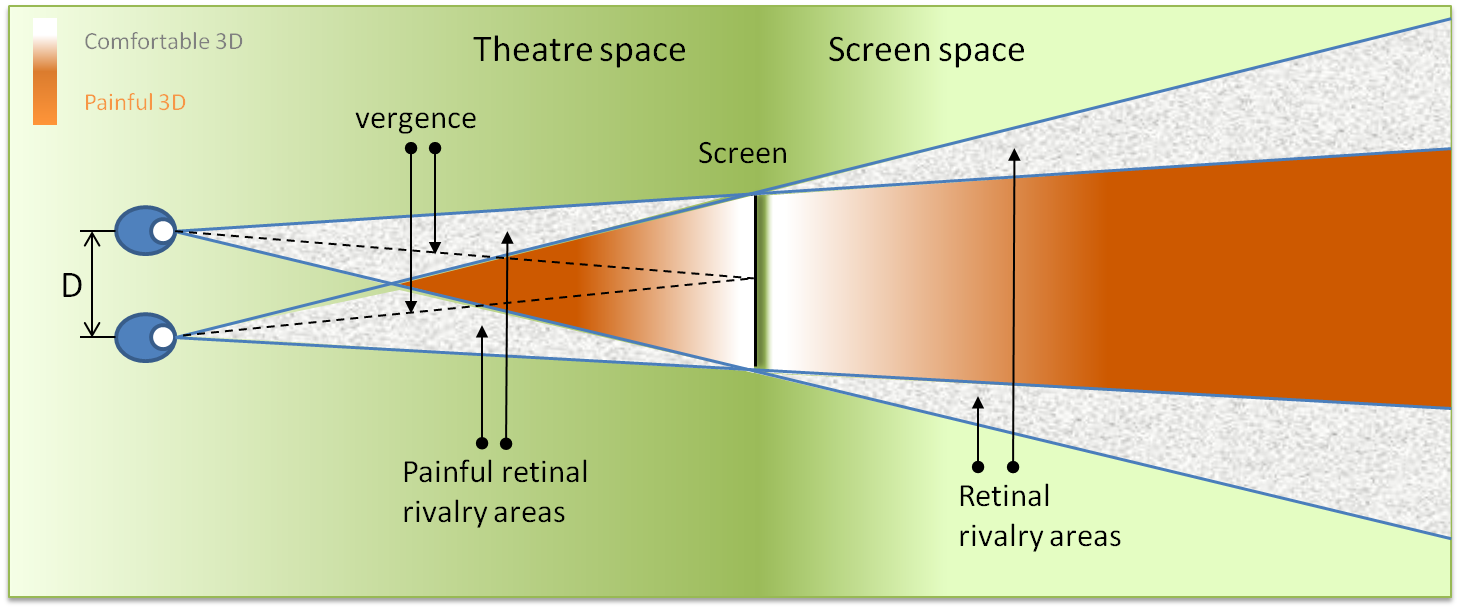
\includegraphics[width=1.0\textwidth]{Stereoscopic_comfort_zone.png}}
\caption{\textit{something... \cite{bib:video_production}} \label{fig:Stereoscopic_comfort_zone}.}
\end{figure}



\begin{figure}[ht]
\centerline{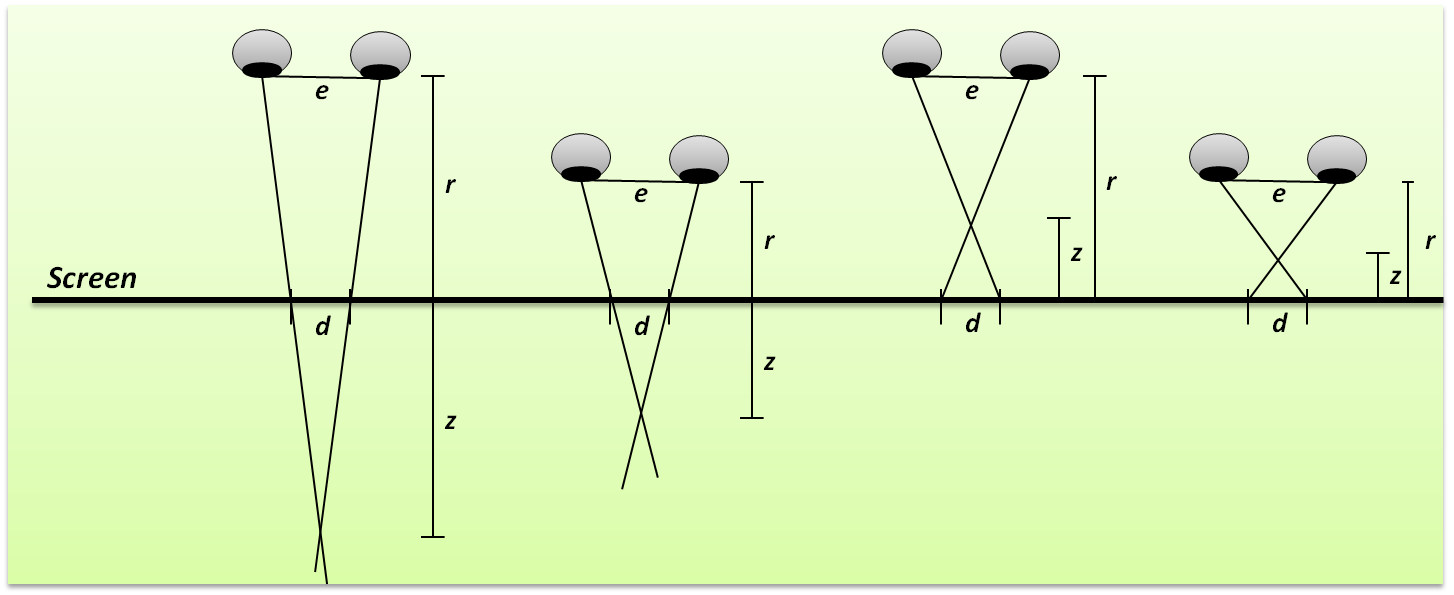
\includegraphics[width=1.0\textwidth]{depth_Vs_viewing_distance.png}}
\caption{\textit{depth Vs viewing distance... \cite{bib:video_production}} \label{fig:depth Vs viewing distance}.}
\end{figure}

\section{Effects of improper 3D}
Improper 3D production will stress the viewer i.e. bad viewer experience 



\section{Filtering of depth map}
All work and no play makes Jack a dull boy,All work and no play makes Jack a dull boy,All work and no play makes Jack a dull boy,All work and no play makes Jack a dull boy,All work and no play makes Jack a dull boy...All work and no play makes Jack a dull boy, all work and no play makes Jack a dull boy, all work and no play makes Jack a dull boy.

\subsection{Spatial-Depth super resolution for Range Images}
As discussed in \cite{Spatial_Depth_Super_Resolution}, using one or two registered color images as reference, we can iteratively refine the low-resolution depth map, in terms of both its spatial resolution and depth precision. This whole process is illustrated in the \textit{figure~\ref{fig:chapter2_op}}.

\begin{figure}[ht]
\centerline{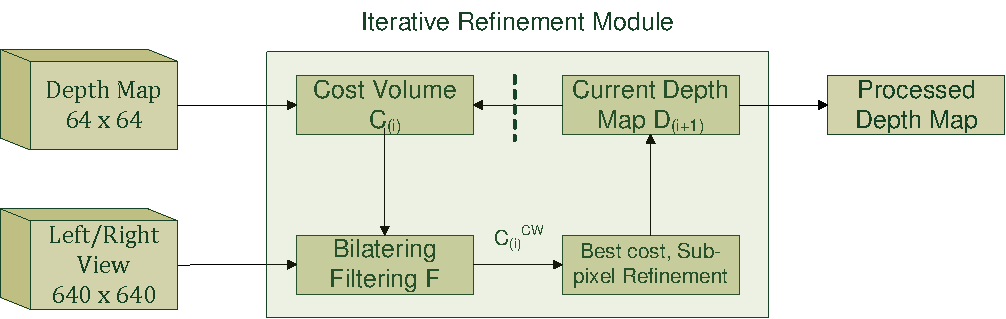
\includegraphics[width=0.9\textwidth]{Spatial_Depth_Super_Resolution_for_Range_Images.pdf}}
\caption[Framework for spatial-depth super resolution for range images]%
{\textit{Framework for spatial-depth super resolution for range images. The range image serves as the initial depth-map hypothesis. Then follows an iterative refinement process. A cost volume is built according to the current depth map hypothesis. A bilateral filter is then applied to the cost volume to avoid the smoothening effect near the depth discontinuities. A winner-takes-all and sub-pixel estimation procedure is used to produce a new depth map hypothesis, which is fed back into the process as described in \cite{Spatial_Depth_Super_Resolution}.}\label{fig:chapter2_op}}
\end{figure}

\paragraph{}
The iterative refinement process has three major steps. First, a cost volume $C_{i}$ is generated from the current depth-map $D_{(i)}$. Second, a Bilateral Filtering is performed for each slice of the cost volume to generate a new cost volume $C_{(i)}^{CW}$. Finally the depth hypothesis with minimal cost is selected and a sup-pixel estimation is applied to obtain the final depth-map $D_{(i+1)}$.

\paragraph{}
Bilateral Filter forms one of the integral part in the iterative refinement process. It has been previously used with great success for stereo algorithms in \cite{Stereo_Matching} and \cite{Adaptive_Support_Weight_Approach}. In the next chapter we will elaborately discuss on this filtering scheme and also show how it's performance can be enhanced using a GPU device.

\section{Transmission of stereo content}
All work and no play makes Jack a dull boy,All work and no play makes Jack a dull boy,All work and no play makes Jack a dull boy,All work and no play makes Jack a dull boy,All work and no play makes Jack a dull boy...All work and no play makes Jack a dull boy, all work and no play makes Jack a dull boy, all work and no play makes Jack a dull boy.
